
\documentclass[tikz,border=2mm]{standalone}
\usepackage[utf8]{inputenc}
\usepackage[T1]{fontenc}
\usepackage{amsmath}
\usepackage{amssymb}
\usetikzlibrary{arrows.meta,positioning,calc,shapes.geometric}
\usepackage{xcolor}

\definecolor{inkNavy}{HTML}{1B2733}
\definecolor{slate}{HTML}{3B4B5C}
\definecolor{paper}{HTML}{FBFAF7}
\definecolor{amber}{HTML}{C97A2B}
\definecolor{teal}{HTML}{2E7D74}
\definecolor{softred}{HTML}{A6402F}
\definecolor{lightgrey}{HTML}{E7E4DD}
\definecolor{midgrey}{HTML}{8B8A85}

\begin{document}
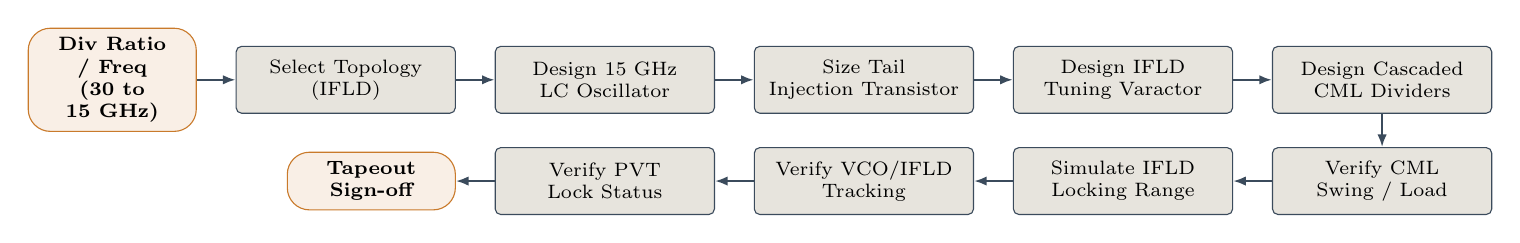
\begin{tikzpicture}[
  node distance=6pt and 14pt,
  box/.style={draw=slate, fill=lightgrey, rounded corners=2pt, text width=2.55cm, align=center, minimum height=0.85cm, font=\scriptsize},
  term/.style={draw=amber, fill=amber!12, rounded corners=8pt, text width=1.9cm, align=center, minimum height=0.7cm, font=\scriptsize\bfseries},
  arr/.style={-{Latex[length=1.6mm]}, slate, thick}
]
\node[term] (spec) {Div Ratio / Freq\\(30 to 15 GHz)};
\node[box, right=of spec] (top) {Select Topology\\(IFLD)};
\node[box, right=of top] (osc) {Design 15 GHz\\LC Oscillator};
\node[box, right=of osc] (inj) {Size Tail\\Injection Transistor};
\node[box, right=of inj] (tune) {Design IFLD\\Tuning Varactor};
\node[box, right=of tune] (cml) {Design Cascaded\\CML Dividers};

\node[box, below=12pt of cml] (swing) {Verify CML\\Swing / Load};
\node[box, left=of swing] (lock) {Simulate IFLD\\Locking Range};
\node[box, left=of lock] (track) {Verify VCO/IFLD\\Tracking};
\node[box, left=of track] (pvt) {Verify PVT\\Lock Status};
\node[term, left=of pvt] (fin) {Tapeout\\Sign-off};

\draw[arr] (spec)--(top); \draw[arr] (top)--(osc); \draw[arr] (osc)--(inj);
\draw[arr] (inj)--(tune); \draw[arr] (tune)--(cml); \draw[arr] (cml)--(swing);
\draw[arr] (swing)--(lock); \draw[arr] (lock)--(track); \draw[arr] (track)--(pvt);
\draw[arr] (pvt)--(fin);
\end{tikzpicture}
\end{document}